\documentclass{article}


\usepackage{../arxiv}

\usepackage[utf8]{inputenc} % allow utf-8 input
\usepackage[T1]{fontenc}    % use 8-bit T1 fonts
\usepackage{hyperref}       % hyperlinks
\usepackage{enumerate}      % pretty enumeration
\usepackage{url}            % simple URL typesetting
\usepackage{booktabs}       % professional-quality tables
\usepackage{amsfonts}       % blackboard math symbols
\usepackage{nicefrac}       % compact symbols for 1/2, etc.
\usepackage{svg}
\usepackage{subcaption}
\usepackage{microtype}      % microtypography
\usepackage{graphicx}
\usepackage{subfiles}

\title{Aphid Detection in Lettuce and Cannabis Leaves}

\subfile{../authors}

\begin{document}
\maketitle

\section{Introduction}
Aphids are small insects that feed on plant sap and can cause significant damage to crops and other plants. 
They can reproduce quickly and produce large populations, making them a persistent problem in agriculture. 
Effective and timely detection of aphids is crucial for controlling their spread and minimizing the damage 
they cause.


Object detection is a task in computer vision that involves locating and classifying objects in images and videos.
It is a complex problem that requires accurate and efficient algorithms to detect objects of interest in a 
cluttered background. In recent years, deep learning techniques have significantly improved the performance 
of object detection algorithms, making them a popular choice for various applications, 
including surveillance, robotics, and agriculture.


The use of object detection algorithms for aphid detection is a relatively new area of research. 
It offers a promising solution for detecting aphids in a more efficient and environmentally friendly 
manner compared to traditional manual inspection and chemical control methods. 
Previous studies have applied object detection algorithms, such as Faster R-CNN, 
to detect aphids on leaves, but there is still room for improvement in terms of accuracy and efficiency.


In this study, we propose a new method for aphid detection using Faster R-CNN with augmentation in the 
contrast of the images. We use a dataset of lettuce leaves to train and evaluate our model. 
Our method aims to improve the results of traditional Faster R-CNN by increasing the contrast of the 
images and making the aphids more distinguishable from the background. Our goal is to provide a 
more efficient and environmentally friendly solution for detecting aphids on leaves.

\begin{figure}[h]
    \centering
    \begin{subfigure}{0.4\textwidth}
        \centering
        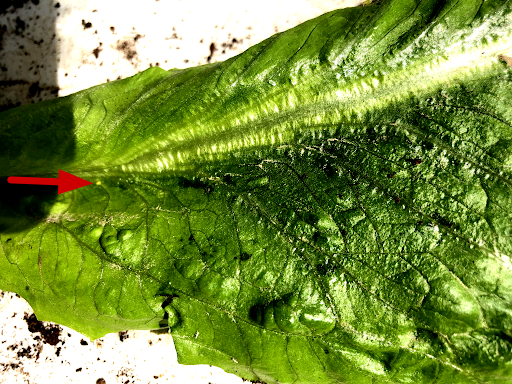
\includegraphics[width=\textwidth]{images/intro_high.png}
        \caption{High contrast image, with augmentation.}
    \end{subfigure}
    \hfill
    \begin{subfigure}{0.4\textwidth}
        \centering
        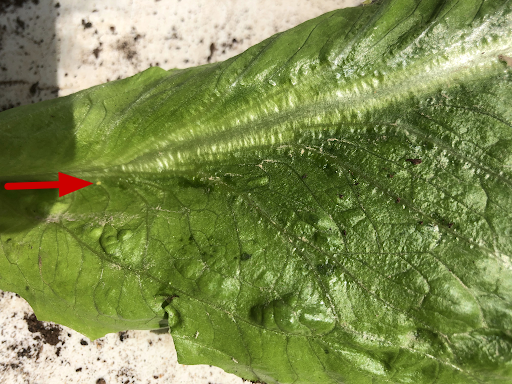
\includegraphics[width=\textwidth]{images/intro_low.png}
        \caption{Low contrast image, without augmentation.}
    \end{subfigure}
    \caption{A comparison showing how contrast can affect the visability of aphics in the image. (aphid is marked with the red arrow)}
\end{figure}

    

\section{Background}
Aphids are a major problem for farmers because they reproduce in days (Chen at al. 2018)
and can infest large fields, causing significant damage to crops. 
This has led to a lot of money being spent on controlling and protecting against 
these pests \cite{CoarseToFine}.


Pest management often involves the use of insecticides, 
which can have adverse effects on crops and the environment. 
However, early detection of infected plants can help reduce the amount of insecticide needed and prevent yield loss. 
Manual techniques for detecting pests require expertise, making them inefficient and 
unreliable \cite{DetectionInWeatFields}. In recent years, digital image analysis and computer vision algorithms 
have been developed to assist with pest detection. By providing images, 
these algorithms can identify the presence of pests and help farmers make more informed decisions 
\cite{DetectionInWeatFields}. These techniques can be more efficient and accurate than manual methods \cite{DetectionInWeatFields}.


Recent advances in object detection have been driven by the success of region proposal methods and 
region-based convolutional neural networks (R-CNNs). 
R-CNN \cite{FasterRCNN}, is a type of object detection algorithm that uses a selective 
search algorithm to generate region proposals, which are candidate regions within an image that 
may contain objects of interest. R-CNN then uses a convolutional neural network (CNN) 
to extract features from the region proposals and an SVM to classify the presence of an 
object within each proposal. Fast R-CNN \cite{FasterRCNN}, 
is a variation of R-CNN that uses a region proposal network (RPN) to generate region proposals, 
making the algorithm faster and more efficient. RPN is a type of neural network used to generate candidate regions, 
or "proposals" within an input image that may contain objects of interest. 
Fast R-CNN is able to run at around 5-10 frames per second, depending on the size of the image 
and the number of region proposals. While it is faster than R-CNN, it may still be too slow for some 
real-time applications. Faster R-CNN \cite{FasterRCNN}, 
further improves upon Fast R-CNN by combining the region proposal network and the CNN into a single network. 
Faster R-CNN can run at around 7-10 frames per second, depending on the size of the image and 
the number of region proposals. YOLO (You Only Look Once) \cite{YOLO}, 
is a type of object detection algorithm that is faster and more efficient than many other algorithms. 
However, it needs to catch up to state-of-the-art detection systems in terms of accuracy. 
While it can quickly identify objects in images, it needs help to localize small objects precisely. 
Despite this limitation, YOLO has been widely adopted in computer vision for its ability to detect 
objects in images and videos efficiently.


Our work will build upon the work done in image detection and aphid detection, 
we will use the Faster-RCNN model with the addition of domain-specific pre-processing 
like removing images which have less than k\% green pixels, where k is a hyper-parameter.

\section{Related Work}
There are many challenges in automatically detecting aphids. 
Here, we review some methods and specific problem formulations for aphid detection. 
These methods will try to frame aphid detection differently and define different tasks. 
These methods all try to solve similar problems with aphid detection, 
like the inability of object detection models to detect very small objects in dense clusters.


Ruili et al. propose a new multi-branch convolutional neural network (Mb-CNN) 
to improve accuracy in these challenging environments. Mb-CNN gives better results in counting aphids, 
and it was developed with a density map for aphids in densely distributed regions and overlapped areas. 
The main idea of this method is to use a multi-branch CNN framework to generate the density map of 
aphids to estimate their number. The relevance of that method to our research is detecting aphids. 
The sole purpose of the article is to improve number counting. 
It's less relevant to our study because we want to focus on detecting Aphids.


Jianming Du er al. \cite{DenseTinyPest} presents a new problem called densely clustered tiny (DCT) object detection, 
which involves detecting small objects that are densely distributed in small areas. 
The authors argue that existing methods for detecting clustered small objects are not suitable 
for this task and therefore propose a new approach called DCTDet, 
which consists of three core components. The authors evaluate their approach using a specific 
in-field aphid dataset and show that it outperforms existing methods for clustered small 
object detection. The paper's relevance depends on the data set we will use and how aphids are 
localized in it.


Liu et al. (2015) \cite{DetectionInWeatFields} reviews existing techniques for aphid detection, 
such as unsupervised cluster algorithms and image segmentation, 
and proposes a new approach using maximally stable external regions (MSER) based on support 
vector machine and histogram of oriented gradient (HOG) methods. 
Our research is similar in that it uses MSER and HOG in the preprocessing phase, 
but it differs in using the Faster RCNN algorithm for aphid detection.


Rui et al \cite{CoarseToFine} propose a noval method that relays on the distribution of aphids in an image. 
The authors note densely distributed aphids may be harder to detect than well-separated aphids. 
The method suggests localizing the regions of aphid cliques containing a large number of 
aphids and then refining them into single objects. This method is called 
Coarse-to-Fine Network (CFN) and can improve the detection accuracy of aphids in dense 
distribution regions. Our method focuses more on the pre-processing of the data. 
We don't need to localize each aphid, we only check if they exist, and thus the Coarse-to-fine 
approach won't improve our results.

\section{Empiracal Evaluation}
In our experiments we try to answer the question “Can Data Augmentations Improve Faster-RCNN Performance In Aphid Identification on Plants?”
We performed both offline experiments, training deep learning models and comparing thier metrics
, and a user study to further evaluate our method with input from a study group. 

\subsection{Offline Experiment}
We compare an existing Faster-RCNN model with our own model, which uses the augmentation described in our method (contrast adjustment).
Our experiment is done on the Lettuce Photos data set, which contain photos of lettuce and cannabis leaves with and without aphids on them, 
annotated with their class (aphids or no aphids) and bounding boxes for the aphids (see \ref{fig:dataset}).
We took all those photos and divide them into training and testing sets. The data is devided into 80\% trining data and 
20\% testing data.


\begin{figure}
    \centering
    \begin{subfigure}{0.4\textwidth}
        \centering
        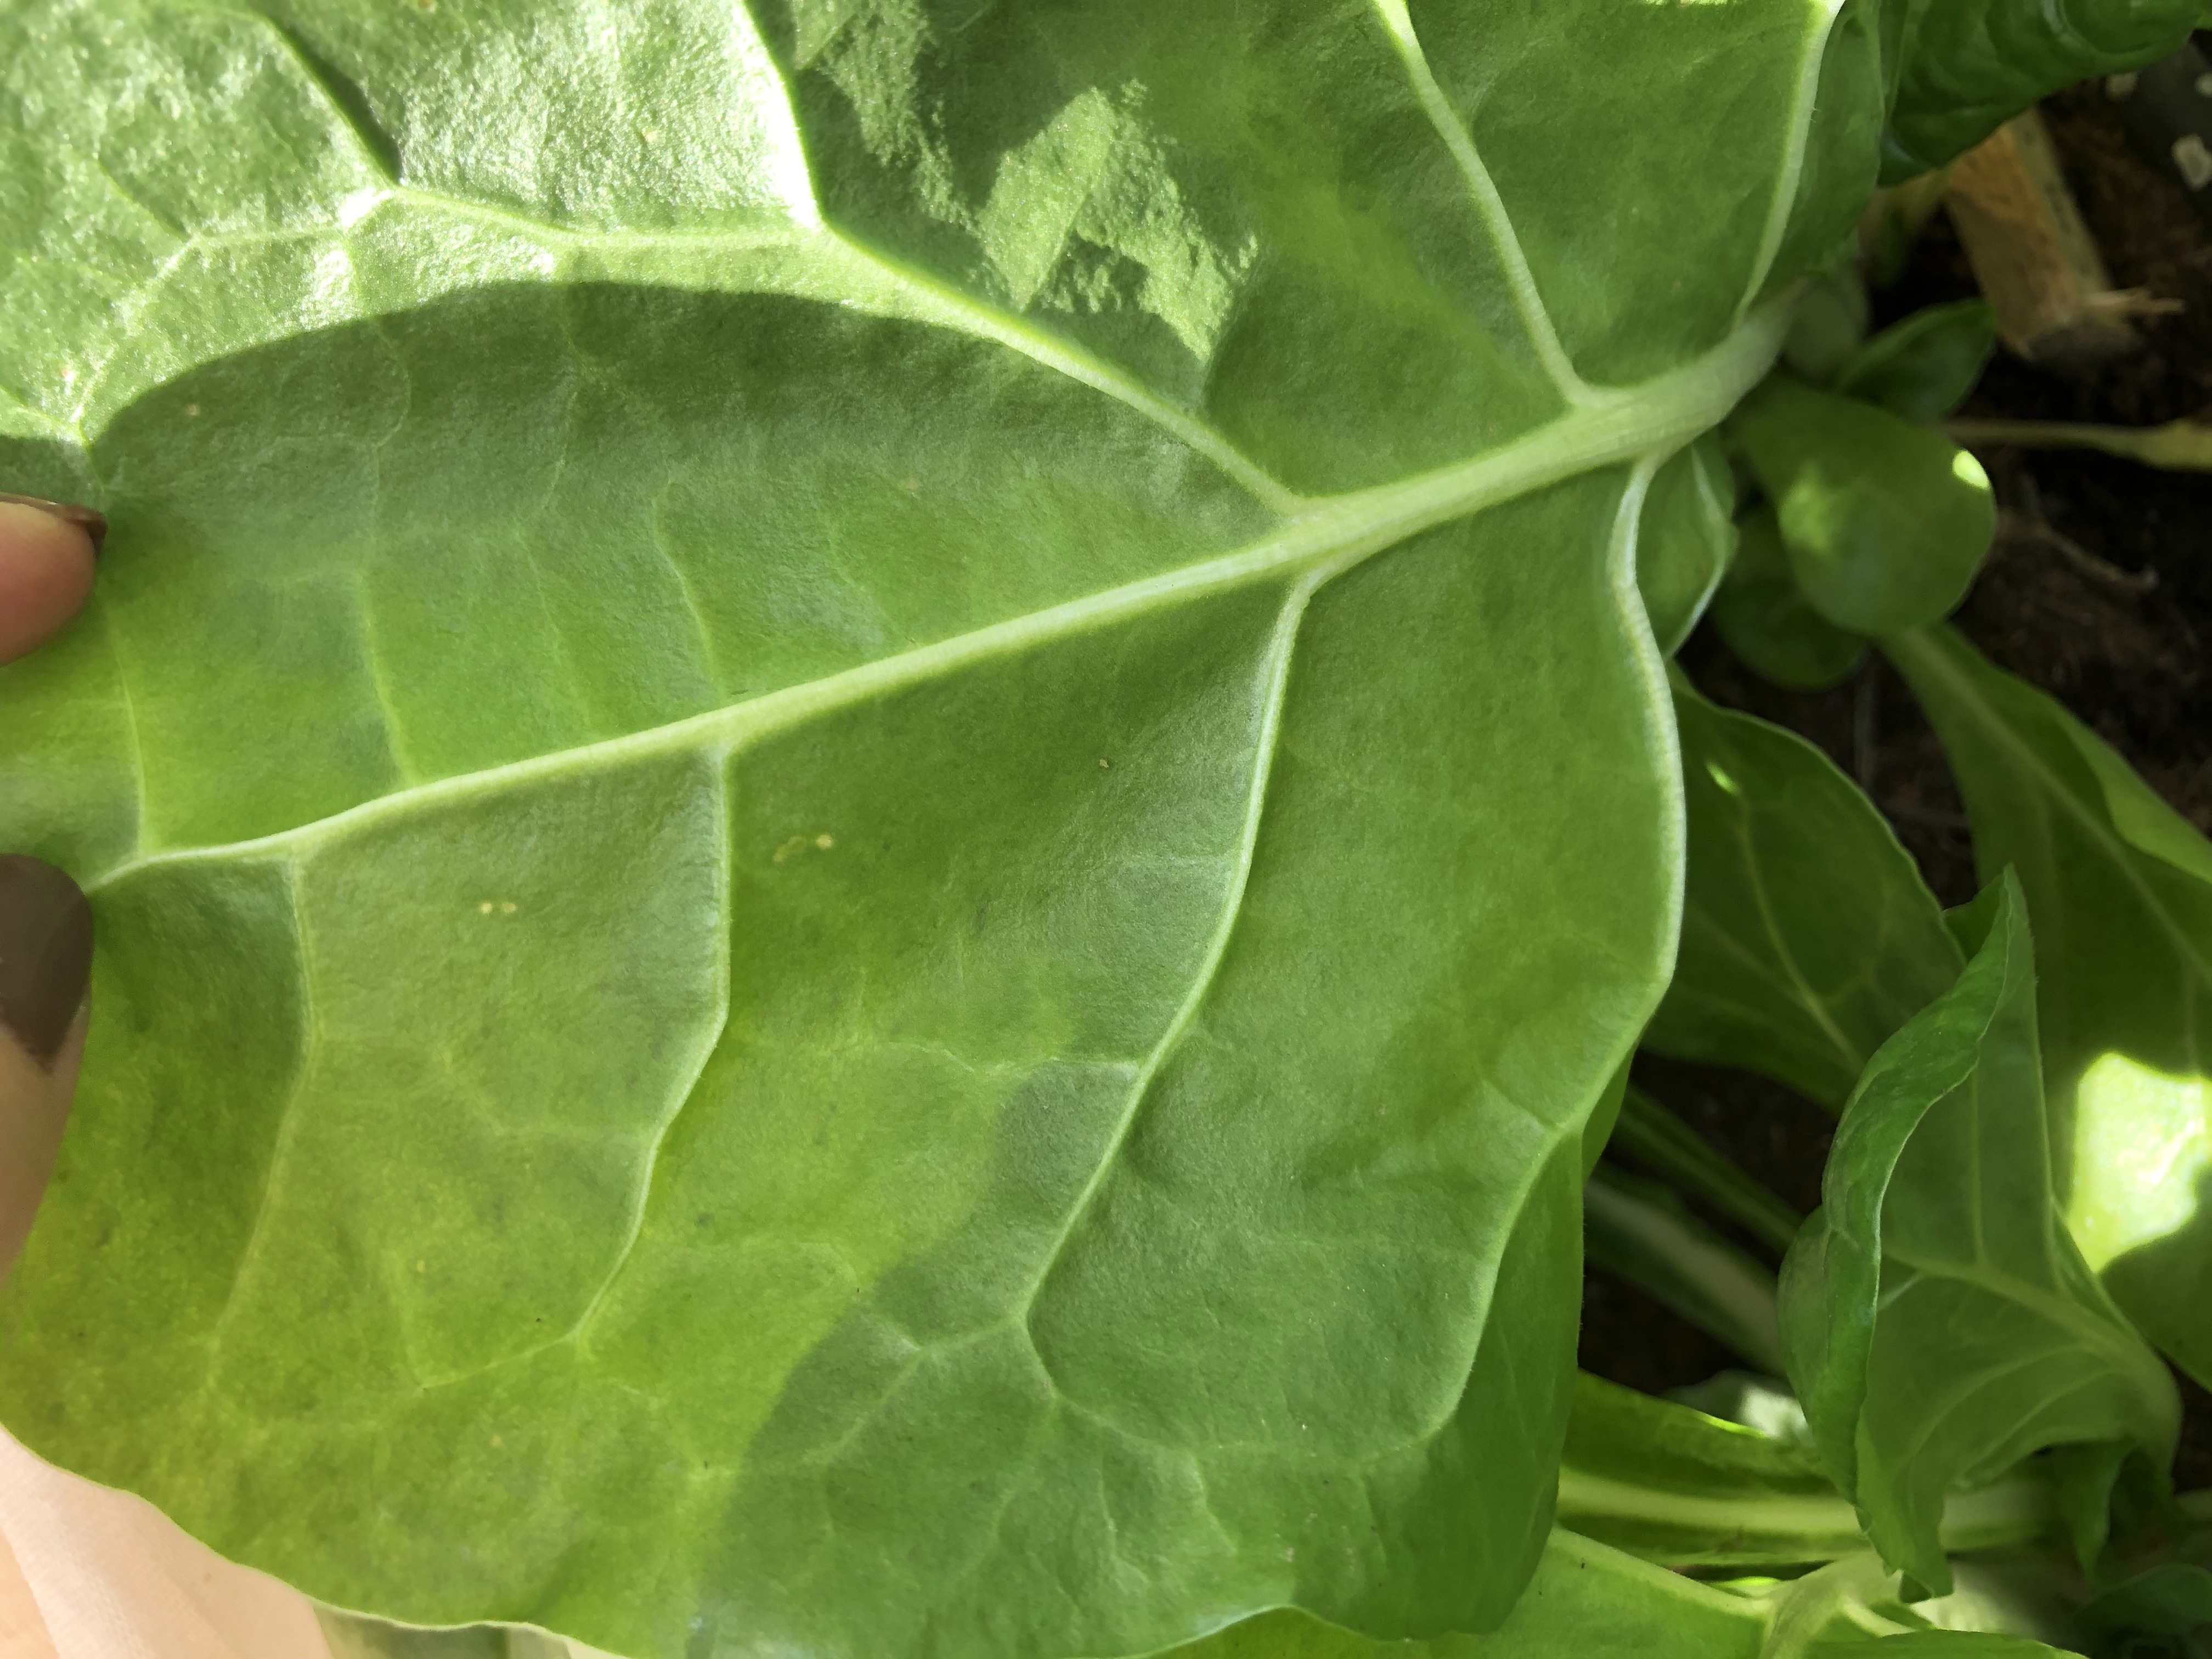
\includegraphics[width=\textwidth]{images/ds1.jpg}
    \end{subfigure}
    \begin{subfigure}{0.4\textwidth}
        \centering
        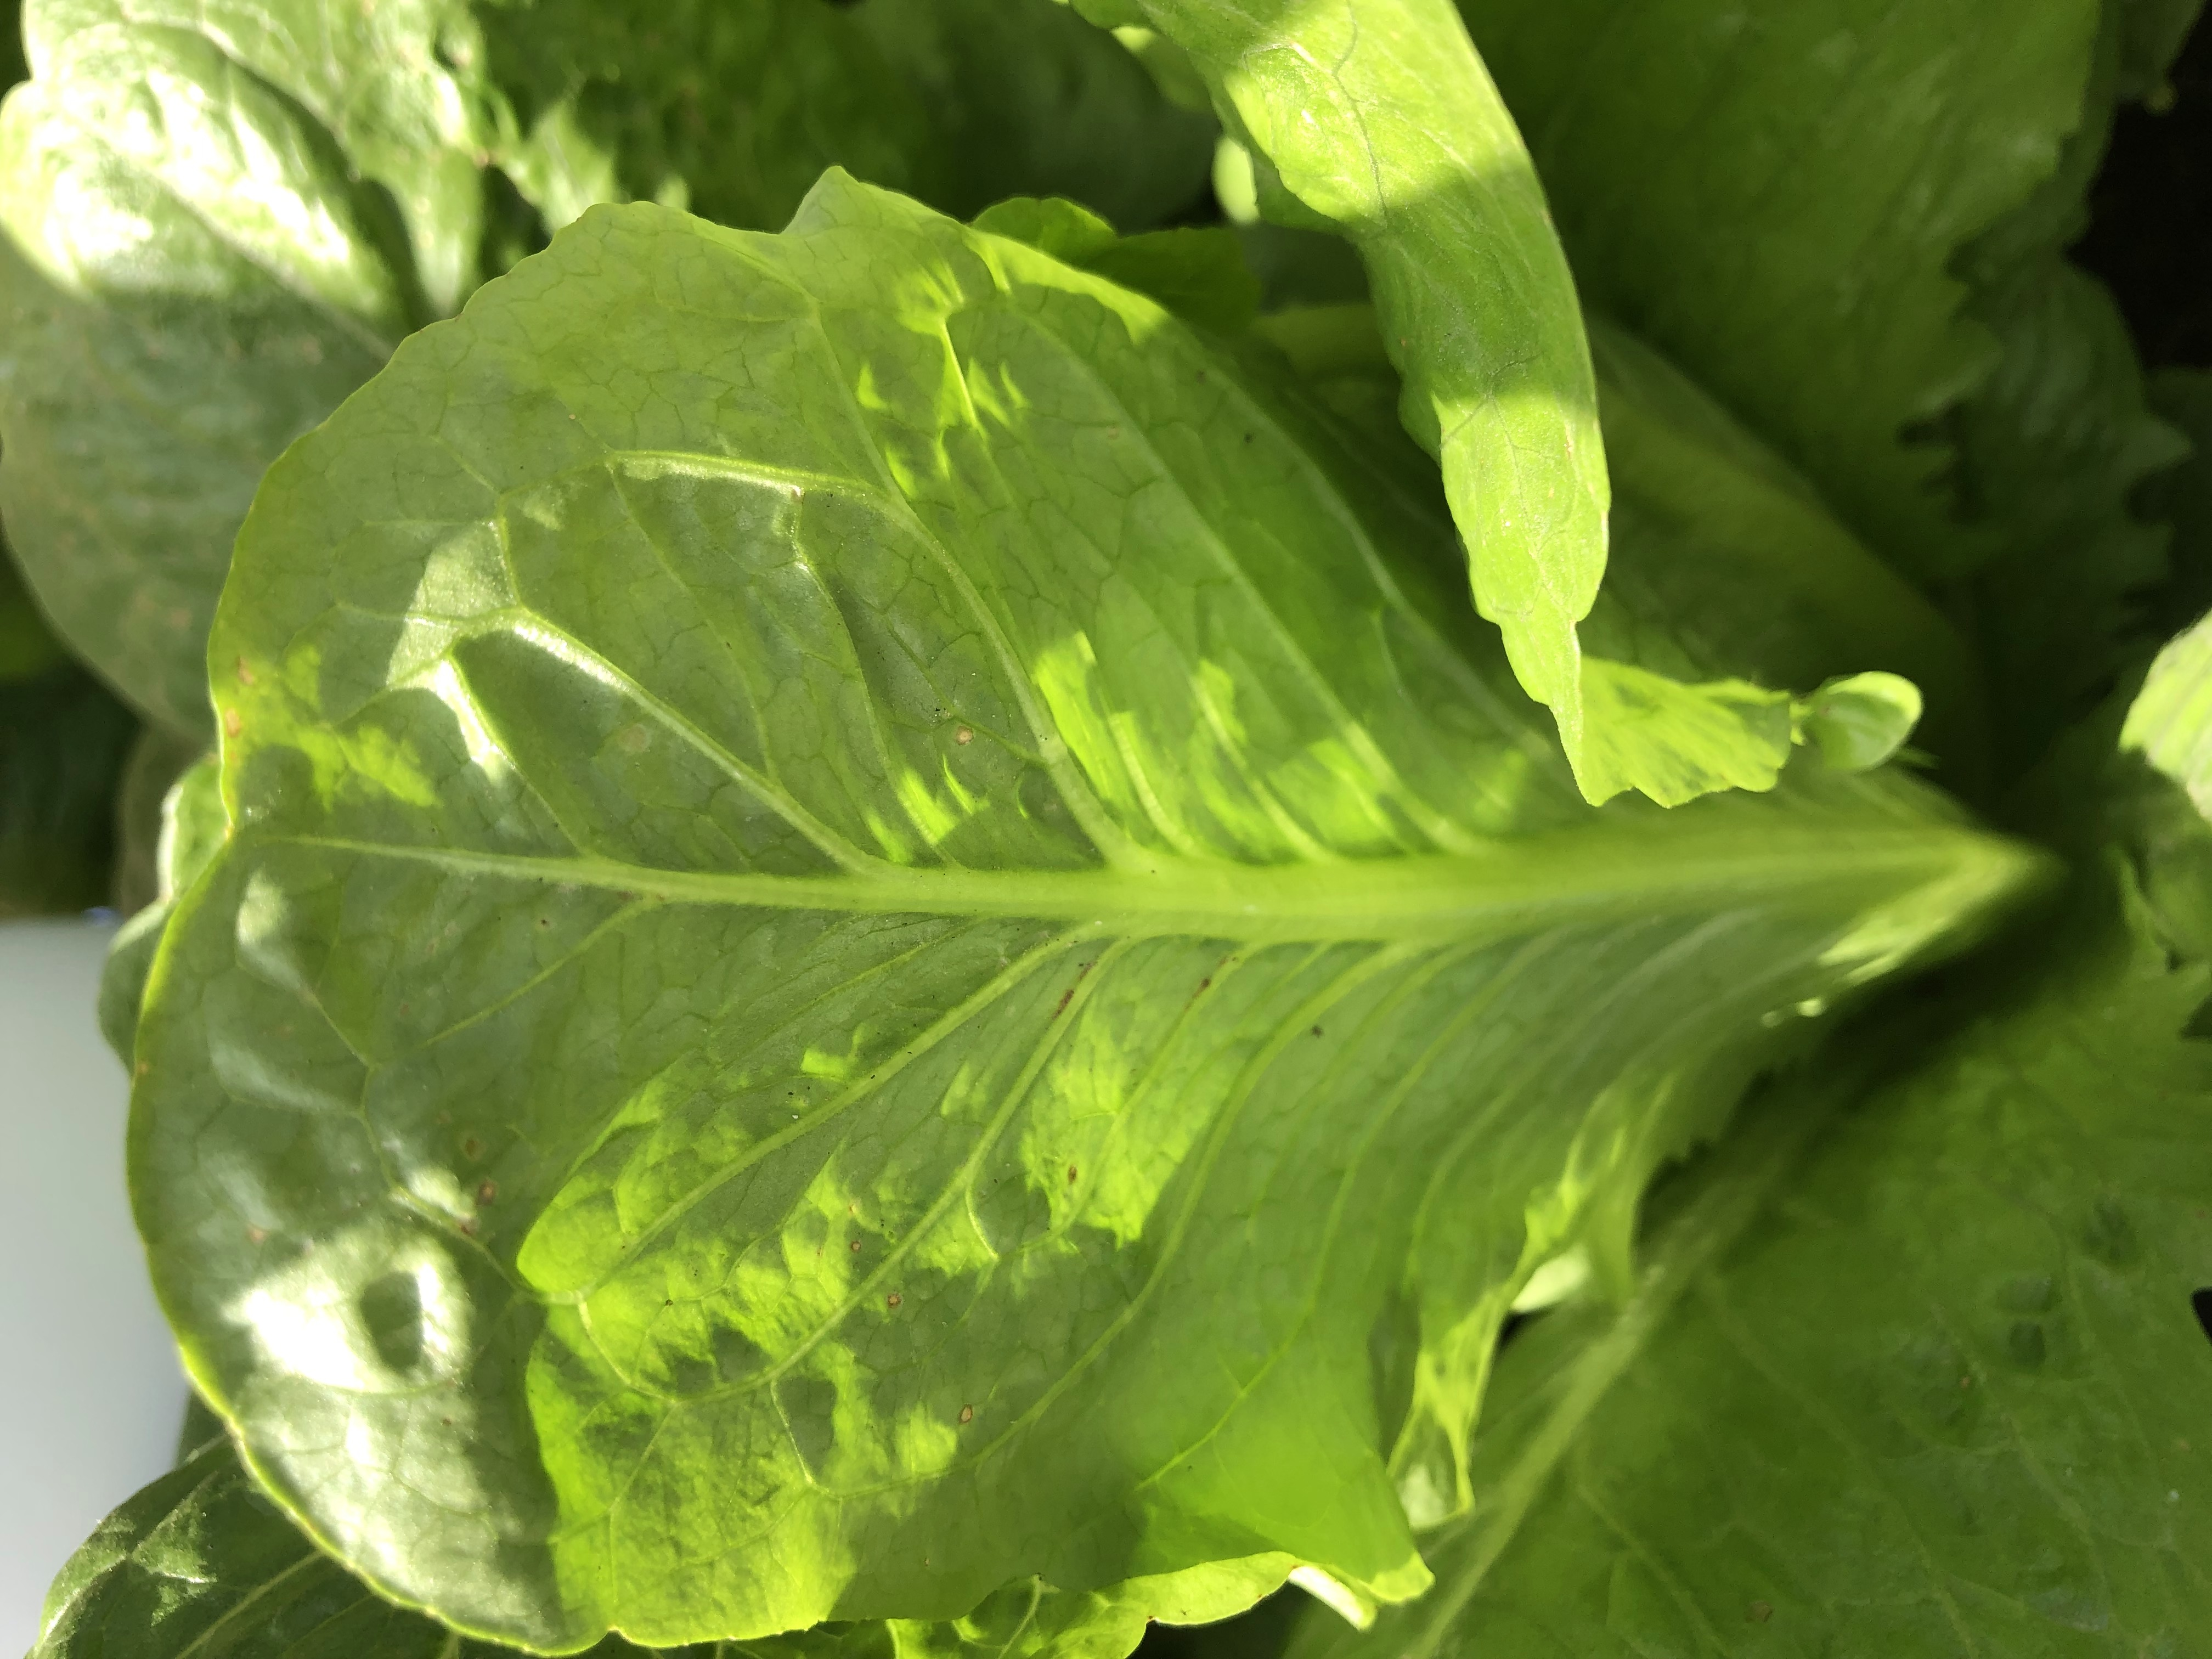
\includegraphics[width=\textwidth]{images/ds2.jpg}
    \end{subfigure}
    \begin{subfigure}{0.4\textwidth}
        \centering
        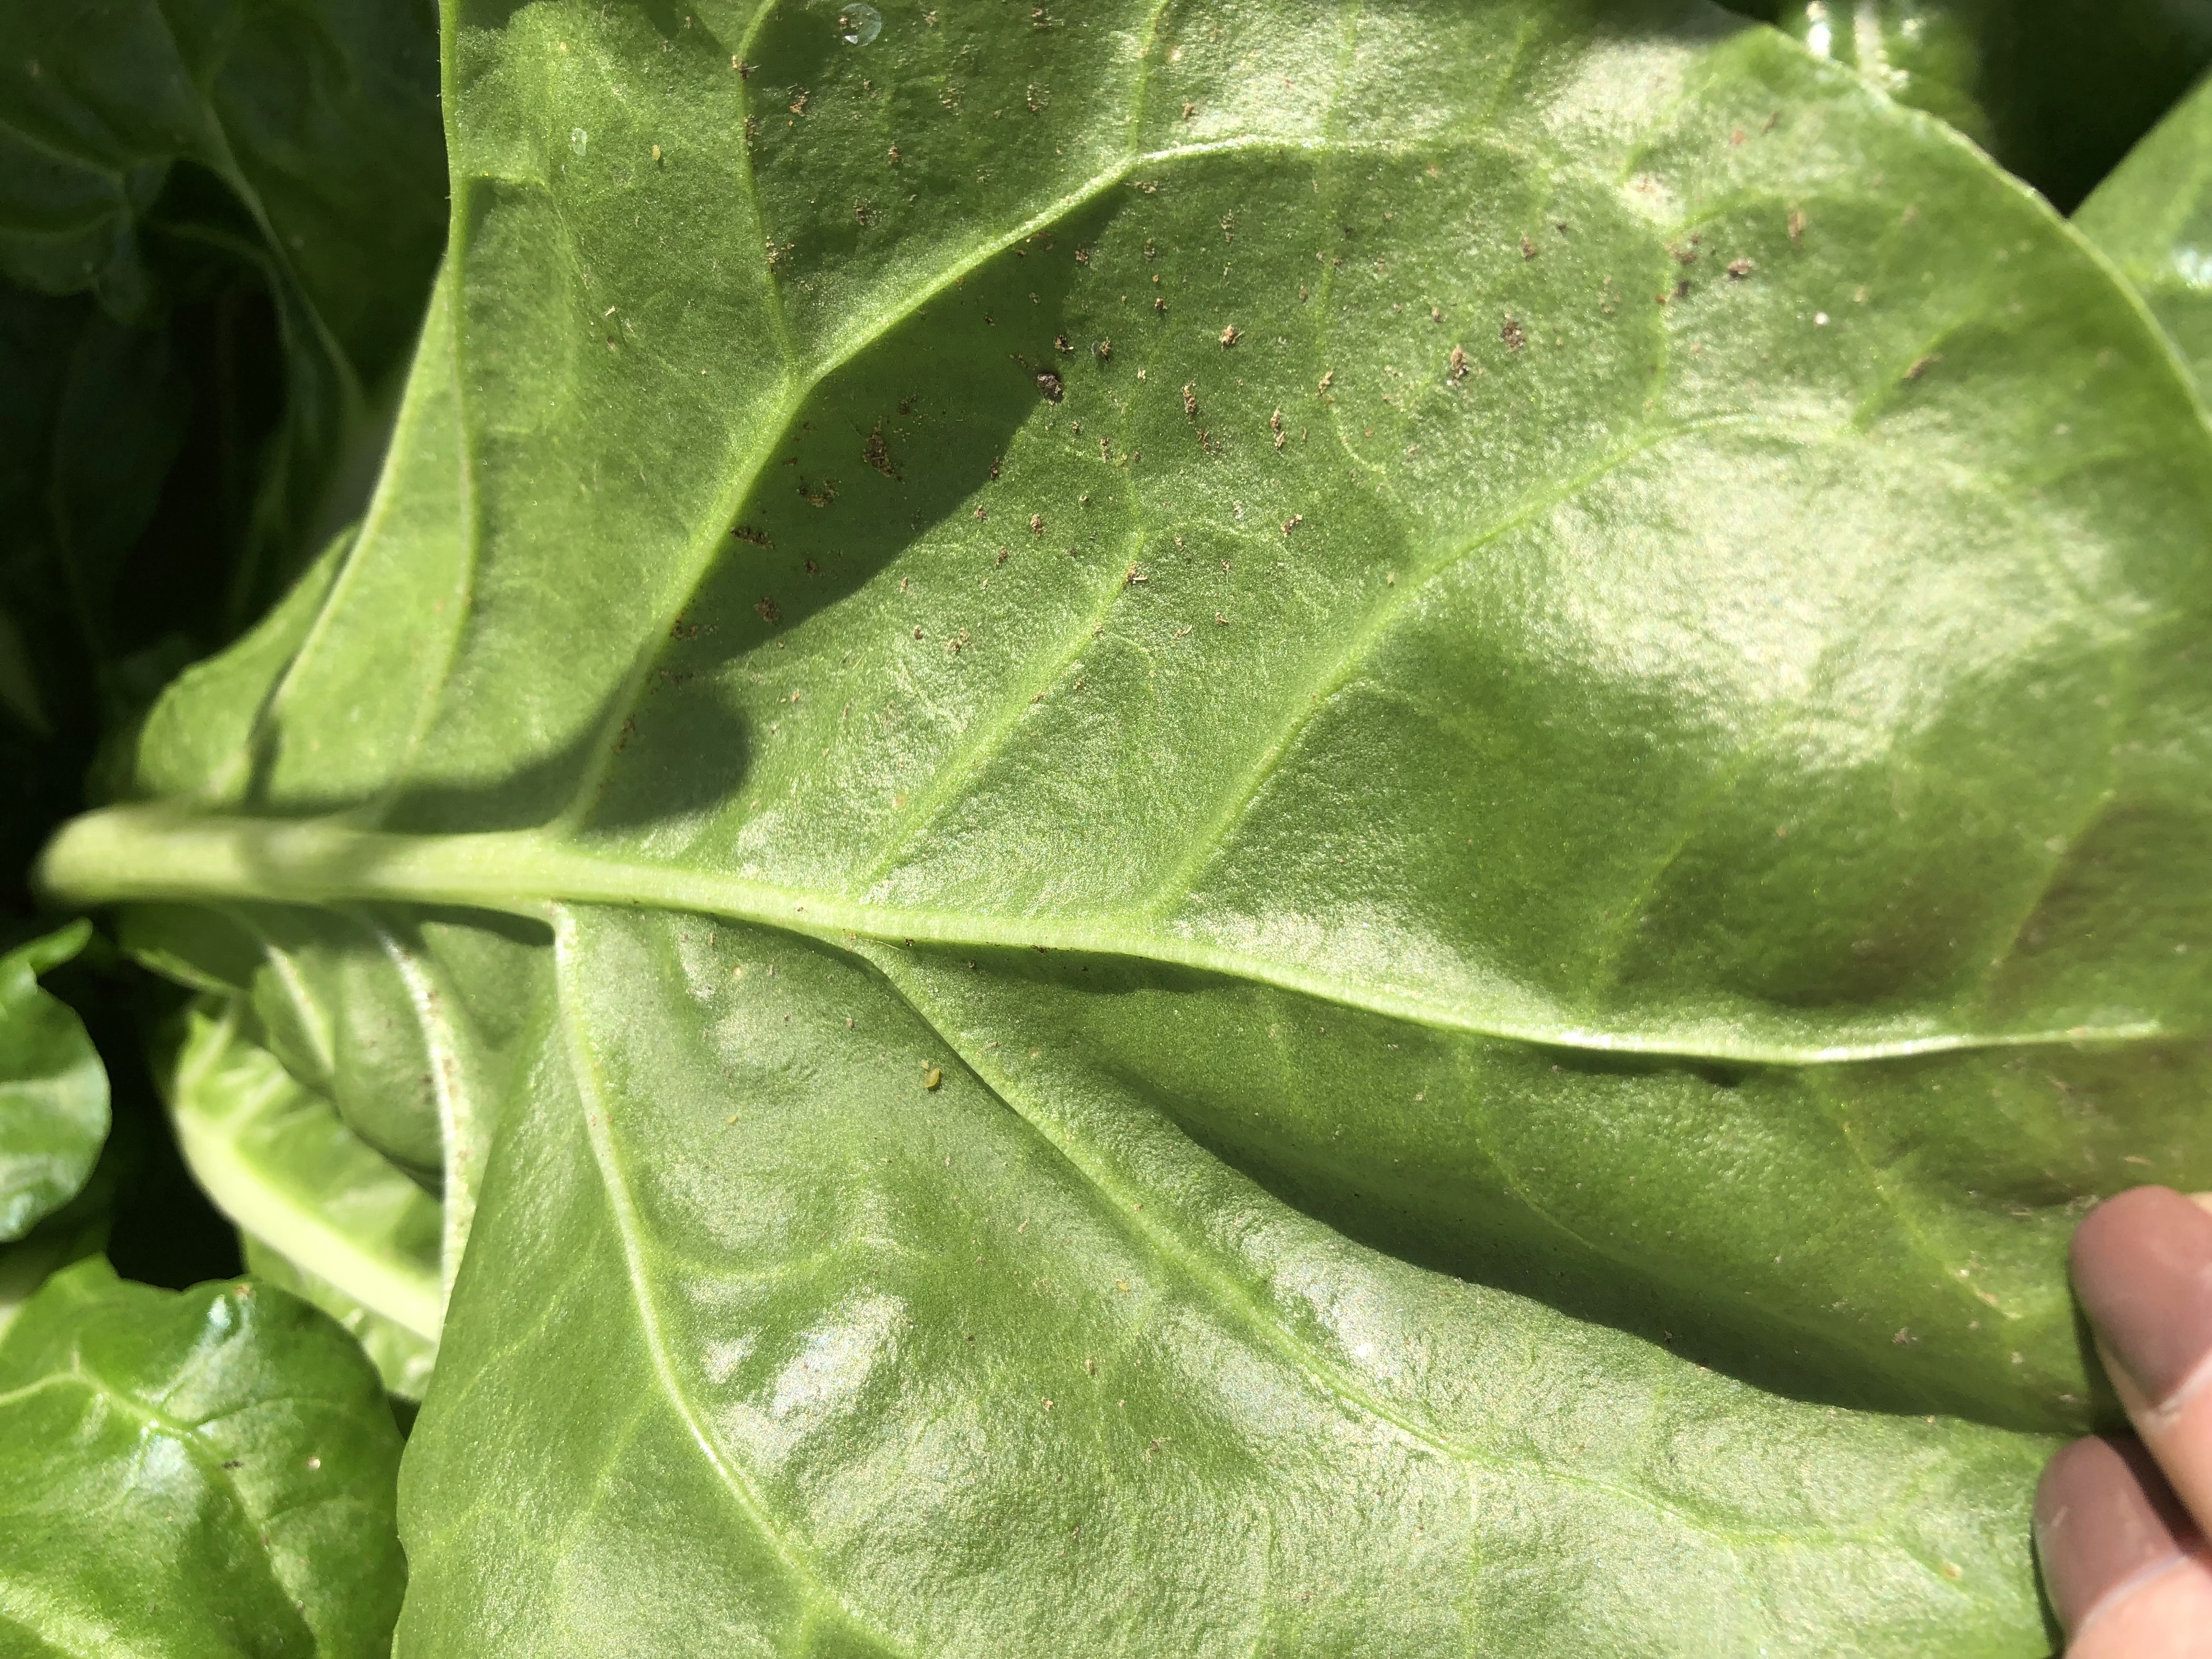
\includegraphics[width=\textwidth]{images/ds3.jpg}
    \end{subfigure}
    \begin{subfigure}{0.4\textwidth}
        \centering
        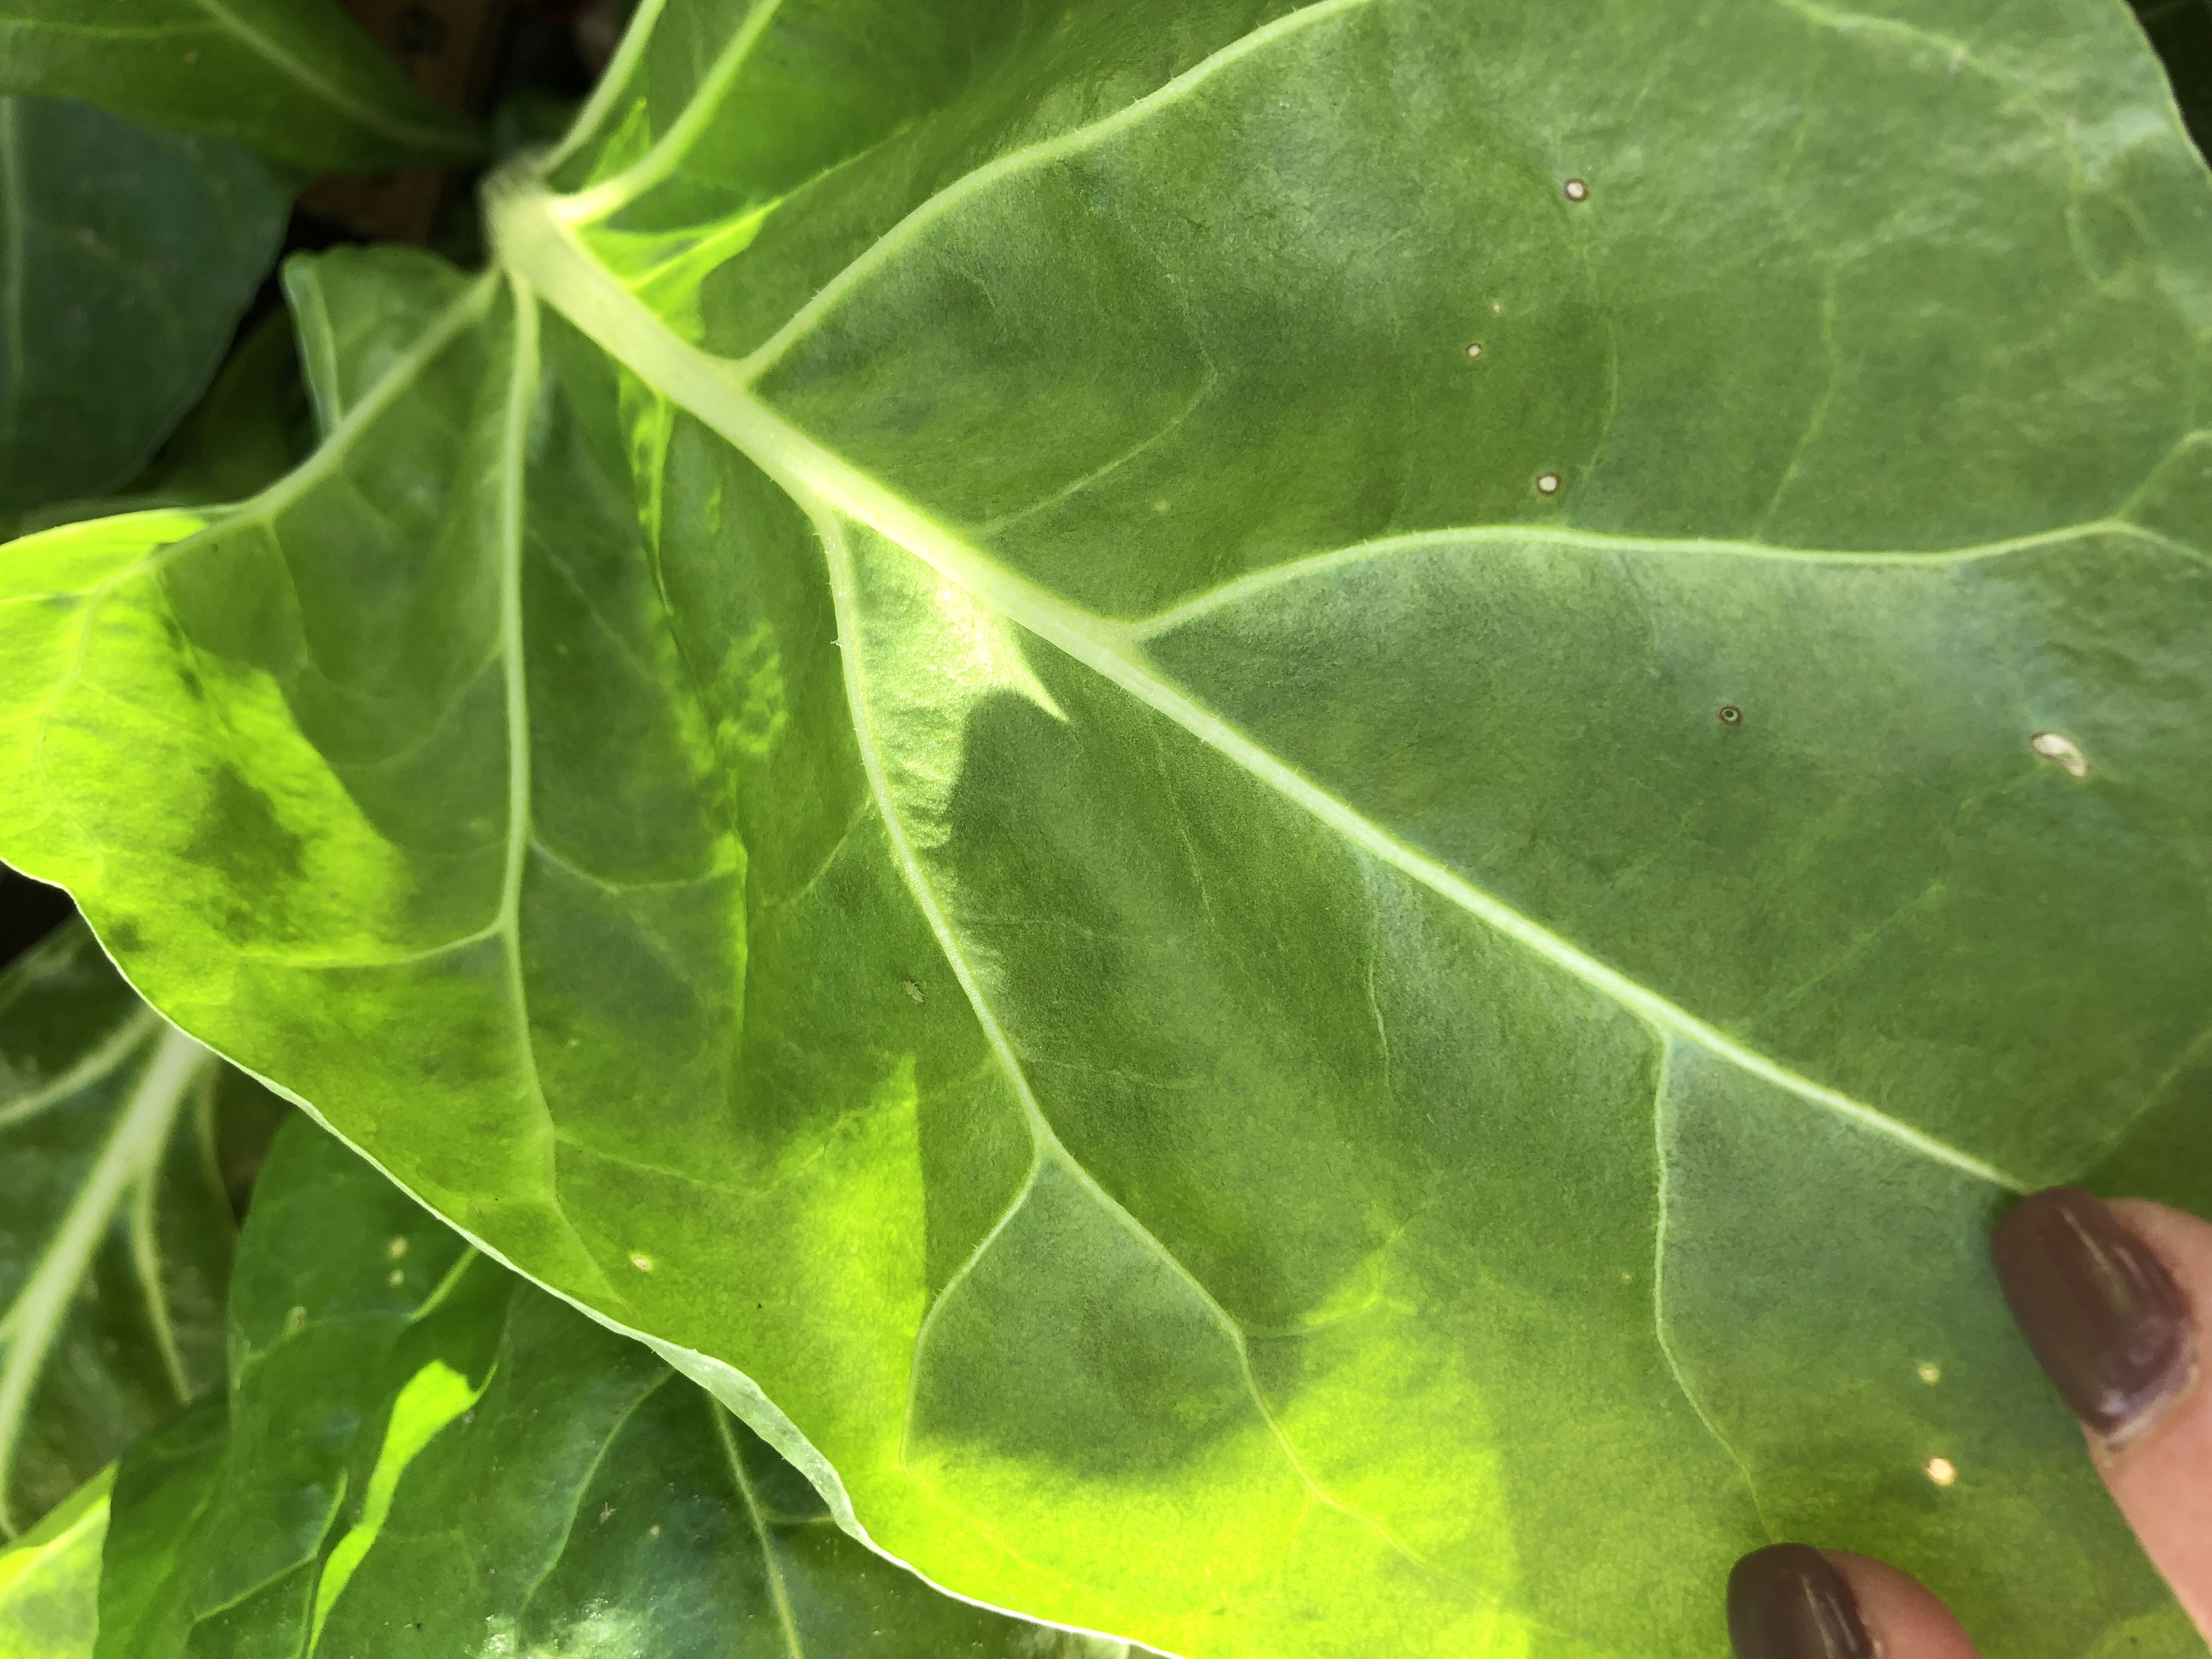
\includegraphics[width=\textwidth]{images/ds4.jpg}
    \end{subfigure}
    \caption{Sample of images from the lettuce aphids dataset.}
    \label{fig:dataset}
\end{figure}

Our model is a binary classifier, we will use precision, recall, and accuracy, to evaluate the model, we compare the models using a precision-recall curve \ref{pr_curve},
showing a more in-depth image of the performance due to the imbalance of the negative class (no aphid) compared to the positive class.
To show that our model significantly improves on the current state of the art we performed Student’s t-test. 
In the case of our experiment, the null hypothesis is that there is no difference between the performance of the models 
detection model as is and the performance of the model after applying augmentation on the data and fine-tuning the original model. 
The alternative hypothesis is that there is a significant difference in performance between the two versions of the model.
We the result in table \ref{t_test_table}

To conduct the t-test, we would need to gather data on the performance of the two versions of the model. This will involve running the 
models on a set of test data and measuring performance metrics, such as precision, recall, and accuracy 
(as described in section d). Then we would calculate the means of the performance metrics for each version of the 
model and use the t-test to determine whether there is a statistically significant difference between the means.
If the t-test shows a significant difference between the means of the two groups, it would suggest that applying 
augmentation and fine-tuning the model has positively impacted that performance. If the t-test does not show a 
significant difference, it would suggest that the augmentation and fine-tuning have not had a significant effect on performance.
Identifying a number of specific cases in which one system is better than another.
The only way to determine which model is preferable in a given situation is to compare their performance on specific images.
On a specific image, as looking at it, we will see if there is a difference in detecting the objects. Those cases where there will be a difference will be presented.


Finally we performed a sensitivity analysis to evaluate how sensitive our model is to changes in the input variables. In our sensitivity analysis, 
we focued on the effect of contrast on the model’s performance.
We varied the contrast factor from \(0.25\) to \(5\) with jumps of \(0.25\).
For each step in our sensitivity analysis we trained the model using the augmented images and then evaluated the model
on the testing data, we can see the results in \ref*{fig:sensitivity}
In the case of image contrast levels, the sensitivity analysis involved evaluating how the performance of 
the model changed as the contrast levels of the images used to train the model are varied.
To conduct a sensitivity analysis of image contrast levels, we would start by selecting a range of contrast levels to test. 
This will include both low and high contrast levels, as well as a range of intermediate levels. 
Then, we would apply these contrast levels to the images used to train the model, and evaluate the performance of the model on a set of test data after each contrast level is applied.
By comparing the performance of the model at different contrast levels, we can determine how sensitive the model is to changes in contrast level, 
and identify any range of contrast levels that may be particularly beneficial or detrimental to model performance.

\begin{figure}[h]
    \centering
    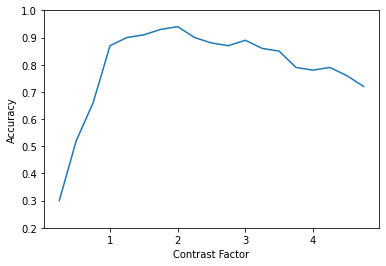
\includegraphics[width=0.6\textwidth]{images/sensitivity.png}
    \caption{Sensitivity analysis on contrast levels.}
    \label{fig:sensitivity}
\end{figure}

\subsubsection{Results}
We managed to show that our method can outperform current state of the art object detectioni methods,
in a robust way, that is statistically segnificant, as is insensitive to small changes in the input.
We were able to identify the aphids with 94\% accuracy on our data set compared to 92\% with the FasterRCNN model.

\newpage
\subsection{User Study}

\subsubsection{User Study Question}
Following is the description of our user studies conducted to compare the contrast of images to detect aphids in the human eye. We elaborate on the study question, tasks given and questionnaires taken by our participants.
\subsubsection{Preliminary Questionnaire}
The preliminary questionnaire will contain the following demographic questions: 

\begin{enumerate}
    \item Age
    \item Gender
    \item Education
    \item Specialization
    \item Former knowledge and Seniority in the field of biology or agriculture
\end{enumerate}

\subsubsection{Tasks}
After delivering the preliminary questionnaires, our participants will be asked to complete the following tasks:

\begin{enumerate}
    \item Participants will be presented with ten pre-selected sets of two images. one is the actual image, and the second is the contrast-augmented image.
    Choose which of the images did you find it easier to detect the aphids.
    \item The participant will be asked to justify his/her choice
    \item Participants will be asked to rate the difficulty of the task on a scale of 1 (very easy) to 5 (very difficult).
\end{enumerate}

\subsubsection{Summary Questionnaire}
The summary questionnaire will contain the following questions: 

\begin{enumerate}
    \item In your opinion, how confident are you giving your opinion on the task of favoring one
    images over the other?    
    \item What challenges did you face while choosing which image you prefer?
    \item Do you have any suggestions for improving the study?
\end{enumerate}

\subsubsection{Instructions}
\begin{enumerate}
    \item Participants will be presented with an image and asked to choose which image the prefer to detect the aphids
    \item Participants should use their best judgment and be reassured.
\end{enumerate}

\subsubsection{Discussion on User Study Results}
Our user studies conducted on 10 participants, 3 females and 7 males, on the age of 22 to 31.
The average difficulty of the participants to answer was 2.1 (out of 5).

From the results of the user studies we can observe a slight preference of the participant
towards the contrast-augmented image. Except from one ties for the real image, our participants
preferred the contrast-augmented image. The mean probability to prefer real image is
24\%, hence the probability to prefer contrast-augmented image is 76\%.

\newpage
\bibliographystyle{abbrv}
\bibliography{references.bib}

\end{document}
